\documentclass[12pt,oneside,letterpaper,english]{article}
\usepackage[T1]{fontenc}
\usepackage{graphicx}
\usepackage[latin1]{inputenc}
\usepackage[margin=2.25cm,headheight=26pt,includeheadfoot]{geometry}
\usepackage[english]{babel}
\usepackage{listings}
\usepackage{color}
\usepackage{titlesec}
\usepackage{titling}
\usepackage[framed, numbered]{matlab-prettifier}
\usepackage{changepage}
\usepackage{amsmath}
\usepackage{hyperref}
\usepackage{enumitem}
\usepackage{graphicx}
\usepackage{fancyhdr}
\usepackage{lastpage}
\usepackage{caption}
\usepackage{tocloft}
\usepackage{setspace}
\usepackage{multirow}
\usepackage{titling}
\usepackage{float}
\usepackage{comment}
\usepackage{booktabs}
\usepackage{indentfirst}
\usepackage{lscape}
\usepackage{booktabs,caption}
\usepackage[flushleft]{threeparttable}
\usepackage[english]{nomencl}
\usepackage{xcolor}
\usepackage{lipsum}
\usepackage{datetime2}
\usepackage{hyperref}

% --- set footer and header ---
\pagestyle{fancy}
\fancyhf{}

\setlength{\parindent}{2em}
\title{Eigenvalue Calculation} % to reference as \title, dont use \maketitle
\makeatletter\let\Title\@title\makeatother



\lstset{language=Matlab,
style=Matlab-editor,
basicstyle=\normalsize\mlttfamily,
numbers=left,
numberstyle={\scriptsize\color{black}},	% size of the numbers
numbersep=0.5cm											
}

\newlist{steps}{enumerate}{1}
\setlist[steps, 1]{leftmargin=1.5cm,label = Step \arabic*:}
\renewcommand{\headrulewidth}{1pt}
\renewcommand{\footrulewidth}{1pt}
\renewcommand{\rmdefault}{ptm}

%\lhead{\Title}
\rhead{\nouppercase{\rightmark}}
\lhead{\Title}
%\rfoot{\includegraphics[height=1.5cm]{root/OSUheader.png}} % right header logo
\setlength\headheight{16pt}
\setlength{\footskip}{50pt}
\lhead{\Title} %rightH title
\cfoot{\thepage}

% --- End of page settings ---



\begin{document}
\pagenumbering{roman} 

\begin{titlepage}
\begin{center}
\vspace{2cm}
%\textsc{Oregon State University}\\[1.5cm]

\includegraphics[width=0.3\textwidth]{root/iith logo.png}~\\[1cm]
\vspace{2cm}

% Title
\hrule
\vspace{.5cm}
{ \huge \bfseries Eigenvalue Calculation} % title of the report
\vspace{.5cm}

\hrule
\vspace{1.5cm}

\textsc{\textbf{Author}}\\
\vspace{.5cm}
\centering

% add your name here
Ronit Ranjan \\
AI24BTECH11028

\vspace{4cm}

\centering \today % see latexmkrc for time zone change
\end{center}
\end{titlepage}

\newpage
\tableofcontents

\newpage
\section{Various Algorithms}
\noindent The thing with calculating eigenvalues of a matrix is that there is no algorithm which can calculate the eigenvalues of all matrices(symmetric and non symmetric) and its very time efficient as well. So a few algorithms i considered after looking up like more than 10 different algorithms are:
\subsection{Divide-and-Conquer Algorithm}
\textbf{Pros:}
\begin{itemize}
    \item It is efficient for large and dense matrices.
    \item Its parallelizable which makes its suitable fro high-performance computing.
    \item Can compute all eigenvalues and eigenvectors
\end{itemize}


\textbf{Cons:}
\begin{itemize}
    \item Can compute eigenvalues of symmetric matrices only.
    \item Complex to implement
    \item Less efficient for smaller matrices
\end{itemize}

\subsection{Jacobi Algorithm}
\textbf{Pros:}
\begin{itemize}
    \item Its simple and easy to implement.
    \item Produces accurate results for symmetric matrices
    \item Focuses on rotations instead of multiplication which is computationally cheaper
\end{itemize}
\textbf{Cons:}
\begin{itemize}
    \item It is computationally expensive for large matrices. It follows $O(n^4)$ if all eigenvalues have to be computed.
    \item It does not work directly for genral matrices
\end{itemize}

\subsection{QR Algorithm}
\textbf{Pros:}
\begin{itemize}
    \item Relatively starightforward.
    \item Works on both symmetric and non symmetric matrices
    \item Gives decent accuracy for Small matrices
\end{itemize}

\textbf{Cons:}
\begin{itemize}
    \item Computationally heavy for big matrices(Time complexity = $O(n^3)$).
    \item Though it works for all matrices, but for non symmetric matrices it converges very slowly.
    \item Can have poor accuracy for matrices that have closed spaced eigenvalues
\end{itemize}

\subsection{QR with Hessenberg Reduction}
\textbf{Pros:}
\begin{itemize}
    \item It is better than QR algorithm because it follows time complexity of $O(n^2)$
    \item Works for general matrices
    \item Can handle both real and complex eigenvalues
    \item Eigenvectors can also be calculated.
\end{itemize}\
\textbf{Cons:}
\begin{itemize}
    \item The initial transformation to Hessenberg form has a computational cost of $O(n^3)$ which might dominate for smaller matrices.
    \item Convergence rate might be slow for matrices with closely spaced eigenvalues.
    \item For small matrices it might not be that efficient.
\end{itemize}

\subsection{QR with householder reflections:}
\textbf{Pros:}
\begin{itemize}
    \item Efficient for Dense matrices
    \item Low memory usage
\end{itemize}
\textbf{Cons: }
\begin{itemize}
    \item It is not very optimized for eigenvalue problems.
    \item For small matrices other algorithms may outperform because of overhead in Householder.
\end{itemize}


\section{Implementing the Algorithm}

\subsection{Attempt 1}
\noindent Spoiler Alert: I failed in implementing this. \\
So the idea was to implement 4 different Algorithm for 4 types of matrices i.e Symmetric/Non Symmetric and Small/Large. So I choose the below Algorithm for each type of matrix.
\begin{table}[!ht]
    \centering
    \begin{tabular}{|l|l|l|}
    \hline
        ~ & Small & Large \\ \hline
        Symmetric & Jacobi & Divide and Conquer \\ \hline
        Non-Symmetric & QR & QR with hessenberg \\ \hline
    \end{tabular}
\end{table} 
\subsubsection{But Why?}
\noindent The thing is no algorithm is completely perfectly in itself. The one that is best among them is QR with hessenberg because it could give all eigenvalues even for medium/large dense matrices, but it has a problem of initial overhead which makes it not that efficient for small matrices. We have Jacobi and QR for small matrices which was much efficient than QR with hessenberg for small matrices. Also I thought it would be fun to implement 4 different algorithm in 4 different C programs and there will be one master program which will take the input and will run the most adequate algorithm based on the user's input. 

\subsubsection{Implementation}
So I wrote all the 4 algorithms in C. The code source is below: 
\begin{enumerate}
    \item \href{https://github.com/igiamronit/Software-assignment/blob/451c51466abd68364a245c534d87f55b77e8d1b8/EigenValue%20Algo/Divide%20and%20Conq/dnc.c}{Jacobi}.
    \item \href{https://github.com/igiamronit/Software-assignment/blob/main/EigenValue%20Algo/qr_algo/qr.c}{QR}.
    \item \href{https://github.com/igiamronit/Software-assignment/blob/main/EigenValue%20Algo/Divide%20and%20Conq/dnc.c}{Divide and Conquer}.
    \item \href{https://github.com/igiamronit/Software-assignment/tree/main/EigenValue%20Algo/qr%20with%20hessenberg}{QR with hessenberg}.
\end{enumerate}
Then I tried making the master C program which will call the others programs. I tried using "system" function in C. So what I planned was I will scan the input, print the input into a .txt file, the suitable program will run based on the input and that program will read the input from the .txt file and will calculate the eigenvalues.

\subsubsection{So what is the problem?}
\noindent Skill issue and Time constraint. I tried making the program, it compiled successfully but i think the value didn't get passed to the respective programs properly due to some pointer issue or something. I tried fixing the issue, but because the deadline was close and I started losing hope and eventually dropped this idea.

\subsection{Attempt 2}
\noindent So after failing in the above task, I attempted this approach using only one Algorithm.
\subsubsection{Algorithm}
\noindent So I am gonna try implementing QR with Hessenberg. Various reasons choosing this algorithm was:
\begin{itemize}
    \item Works for all type of matrices.
    \item Can handle both real and complex eigenvalues.
    \item Ideal for dense matrices when computational efficiency is very critical.
    \item Faster iteration because due to Hessenberg form.
    \item Lower memory usage than QR with Householder Reflection.
\end{itemize}

Code: \href{https://github.com/igiamronit/Software-assignment/blob/main/Software%20assignment/eigen.c}{QR with Hessenberg Reduction}.

\subsection{How does the code work?}
\subsubsection{Libraries}
\begin{itemize}
    \item \texttt{stdio.h} and \texttt{stdlib.h} for input/output.
    \item \texttt{math.h} for mathematical function.
    \item \texttt{complex.h} for calculations in calculating complex eigenvalues.
    \item \texttt{time.h} to measure time to calculate eigenvalues.
\end{itemize}

\subsubsection{Functions}
\begin{itemize}
    \item \texttt{allocate matrix} to allocate memory for a 2D matrix(dynamically).
    \item \texttt{freeMatrix} to free the memory for the matrix when it is no longer needed.
    \item \texttt{hessenbergReduction} to reduce the matrix into Hessenberg form
    \item \texttt{qrDecomposition} to orthogonalize H into Q and R using Householder reflectors.
    \item \texttt{qrIteration} Updates H with $R*Q$(to ensure eigenvalues converge along the diagonal). If the subdiagonal entries are below tolerance, then the iterations stop. If the subdiagonal entries are 0, diagonal elements are real eigenvalues. If subdiagonal entries persist, it extracts complex eigenvalues from $2\times2$ blocks.
    \item \texttt{main function} Takes the size of matrix $(n)$ and the element of the matrix rowise and stores it in array $A$. Finally after using \texttt{hessenbergReduction} and \texttt{qrIteration}, stores the final eigenvalues in an matrix \texttt{eigenvalues}.
\end{itemize}

\subsubsection{Matrix behind it}
The QR algorithm is an iterative method that applies the QR decomposition of a matrix \( A \) and forms a sequence of matrices \( A_k \) defined as:
\[
A_k = Q_k R_k, \quad A_{k+1} = R_k Q_k,
\]
where \( Q_k \) is an orthogonal matrix and \( R_k \) is an upper triangular matrix obtained from the QR decomposition of \( A_k \).

As \( k \to \infty \), the sequence \( A_k \) converges to an upper triangular matrix whose diagonal entries are the eigenvalues of \( A \).

\textbf{Hessenberg Reduction}
The efficiency of the QR algorithm can be greatly improved by reducing the input matrix \( A \) to an upper Hessenberg form before applying the QR steps. A Hessenberg matrix \( H \) is a square matrix with zero entries below the first subdiagonal:
\[
H = 
\begin{bmatrix}
h_{11} & h_{12} & h_{13} & \cdots & h_{1n} \\
h_{21} & h_{22} & h_{23} & \cdots & h_{2n} \\
0 & h_{32} & h_{33} & \cdots & h_{3n} \\
\vdots & \vdots & \ddots & \ddots & \vdots \\
0 & 0 & \cdots & h_{n-1,n} & h_{nn}
\end{bmatrix}.
\]

This transformation is achieved using orthogonal similarity transformations:
\[
H = Q^T A Q,
\]
where \( Q \) is a product of Householder reflectors.

\textbf{Householder Reduction to Hessenberg form}
Given a matrix \( A \), the Hessenberg reduction is performed iteratively. At each step, we eliminate elements below the first subdiagonal using Householder reflectors. Let \( v \) be a vector orthogonal to the subdiagonal elements, and define:
\[
P = I - 2\frac{vv^T}{v^T v}.
\]
The similarity transformation \( A \mapsto P A P^T \) results in a Hessenberg matrix.
At each iteration of the QR algorithm, we decompose the current matrix \( H_k \) into \( Q_k R_k \), where:
\begin{itemize}
    \item \( Q_k \): Orthogonal matrix (product of Givens rotations or Householder reflectors).
    \item \( R_k \): Upper triangular matrix.
\end{itemize}
The updated matrix is then computed as:
\[
H_{k+1} = R_k Q_k.
\]
The QR algorithm, applied iteratively to a Hessenberg matrix, converges to a quasi-upper triangular matrix. For real matrices, this means:
\begin{itemize}
    \item Real eigenvalues appear on the diagonal.
    \item Complex conjugate eigenvalue pairs appear in 2x2 blocks.
\end{itemize}

\subsection{Output}
The program gives 3 things as output
\begin{itemize}
    \item \textbf{Number of Iterations}: Number of QR iterations performed.
    \item \textbf{Time}: Time taken to calculate the eigenvalues.
    \item \textbf{Eigenvalues} in form $a + \iota b$
\end{itemize}

\subsubsection{Example}
\begin{itemize}
    \item \textbf{For a 5x5 matrix:} 
    The data for matrix is \href{https://github.com/igiamronit/Software-assignment/blob/main/Report/Data/matrices/5x5.txt}{5x5 matrix}
    \begin{figure}[h!]
    \centering
    \includegraphics[width=0.6\textwidth]{Data/Images/5x5.png} 
    \caption{Output for 5x5 matrix}
    \end{figure}

    \item \textbf{For a 100x100 matrix: }
    The data for matrix is \href{https://github.com/igiamronit/Software-assignment/blob/main/Report/Data/matrices/100x100.txt}{100x100 MATRIX}
    \begin{figure}[h!]
    \centering
    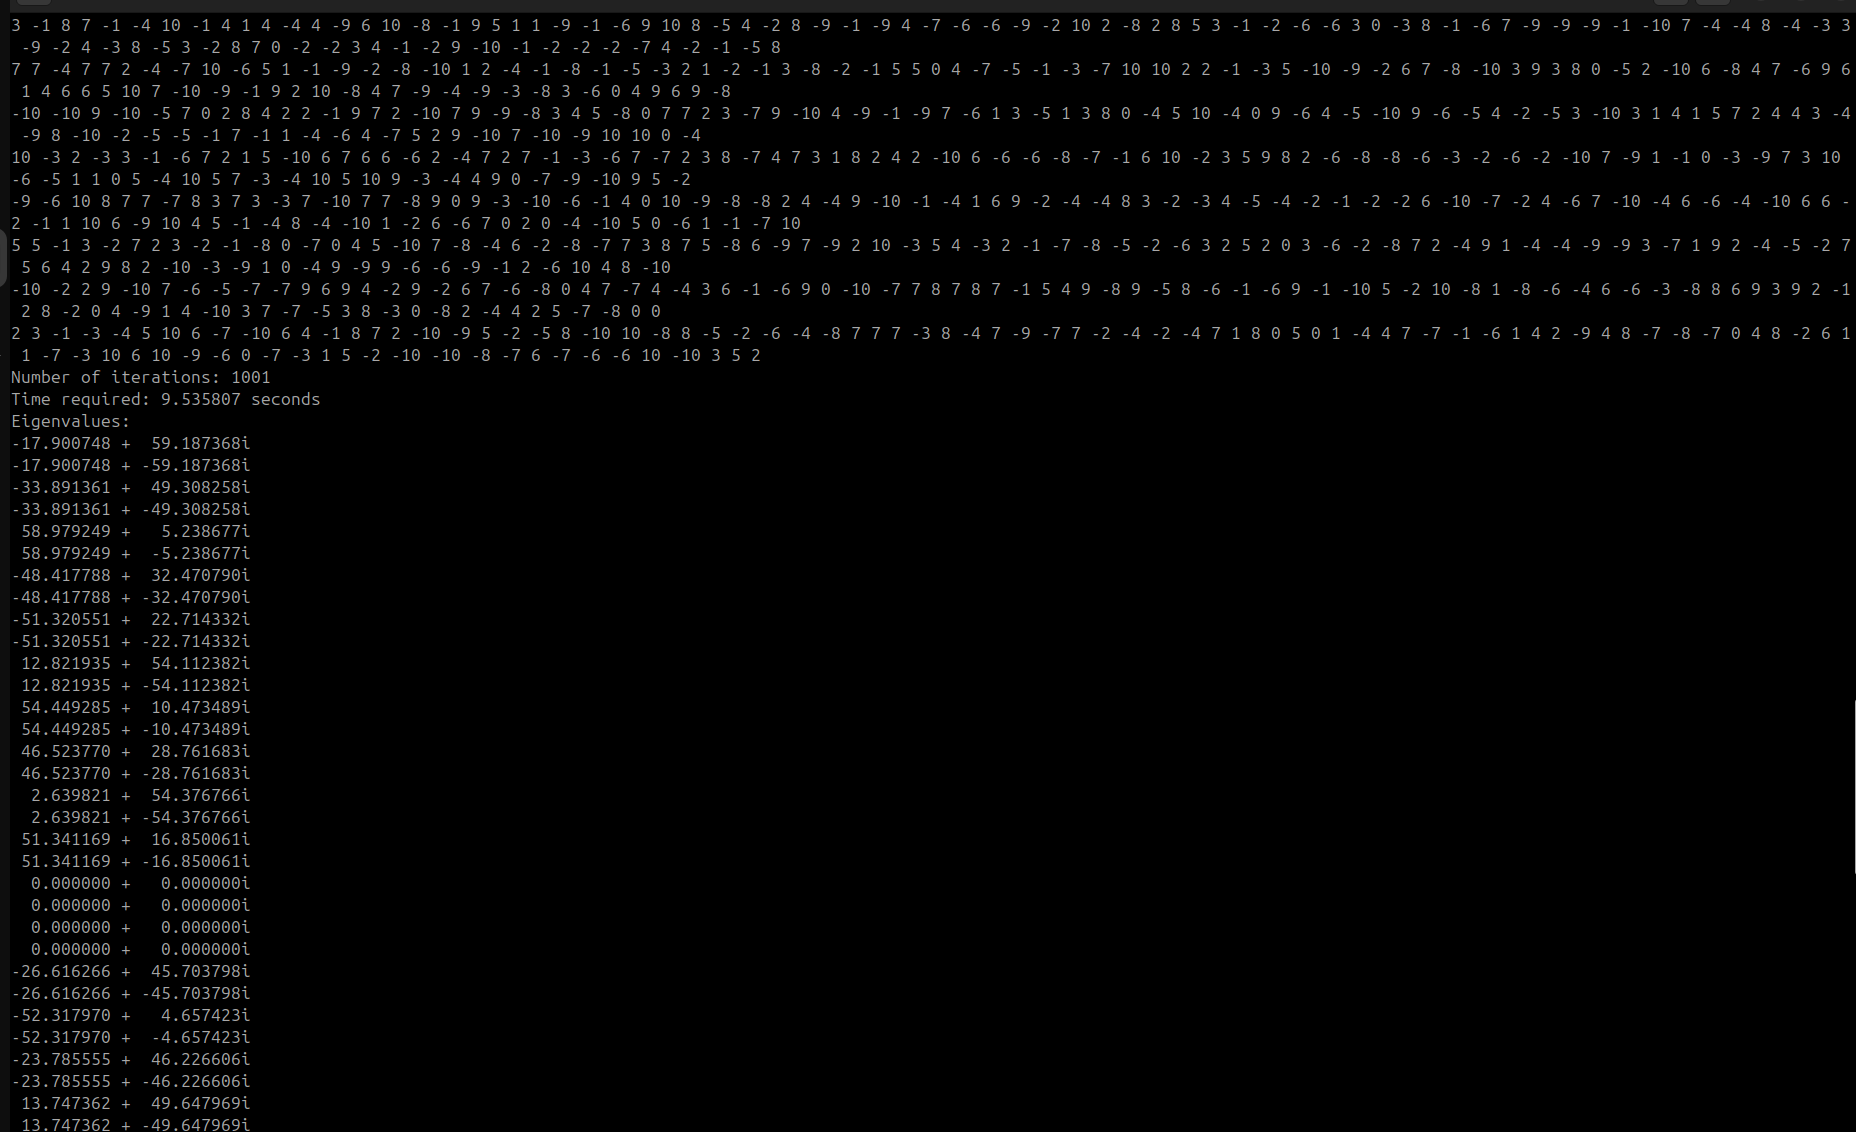
\includegraphics[width=0.6\textwidth]{Data/Images/100x100.png} 
    \caption{Output for 100x100 matrix}
    \end{figure}    
\end{itemize}

















\end{document}

